\documentclass[a4paper]{article}
\usepackage{amsthm}
\usepackage{amsmath} % Define various maths environments
\usepackage{amssymb} % Define various maths symbols
\usepackage{mathrsfs}
\usepackage{geometry} % Adjust the margin, paper size, and etc.
\usepackage{enumerate} % Provide different style of lists
\usepackage{graphicx}
\usepackage{float}
\usepackage{multirow}
\geometry{a4paper,scale=0.78}

\title{—————————————————————————\\ \sc{UM-SJTU Joint Institute}}
\author{\sc{Computer Networks}}
\date{\sc{(Ve489)}\\——————————————————————————————}

\begin{document}
\maketitle
\vspace{5cm}
\centerline{\Large{\sc{Mini-Project 1 Report}}}
\vspace{9cm}
\begin{tabular}{lll}
\qquad \qquad Name: Sun Yiwen&ID: 517370910213\\
\qquad \qquad Date: June 21 2020
\end{tabular}

\newpage
\section{Step 1: Capture a Trace}
\begin{figure}[htbp]
\centering
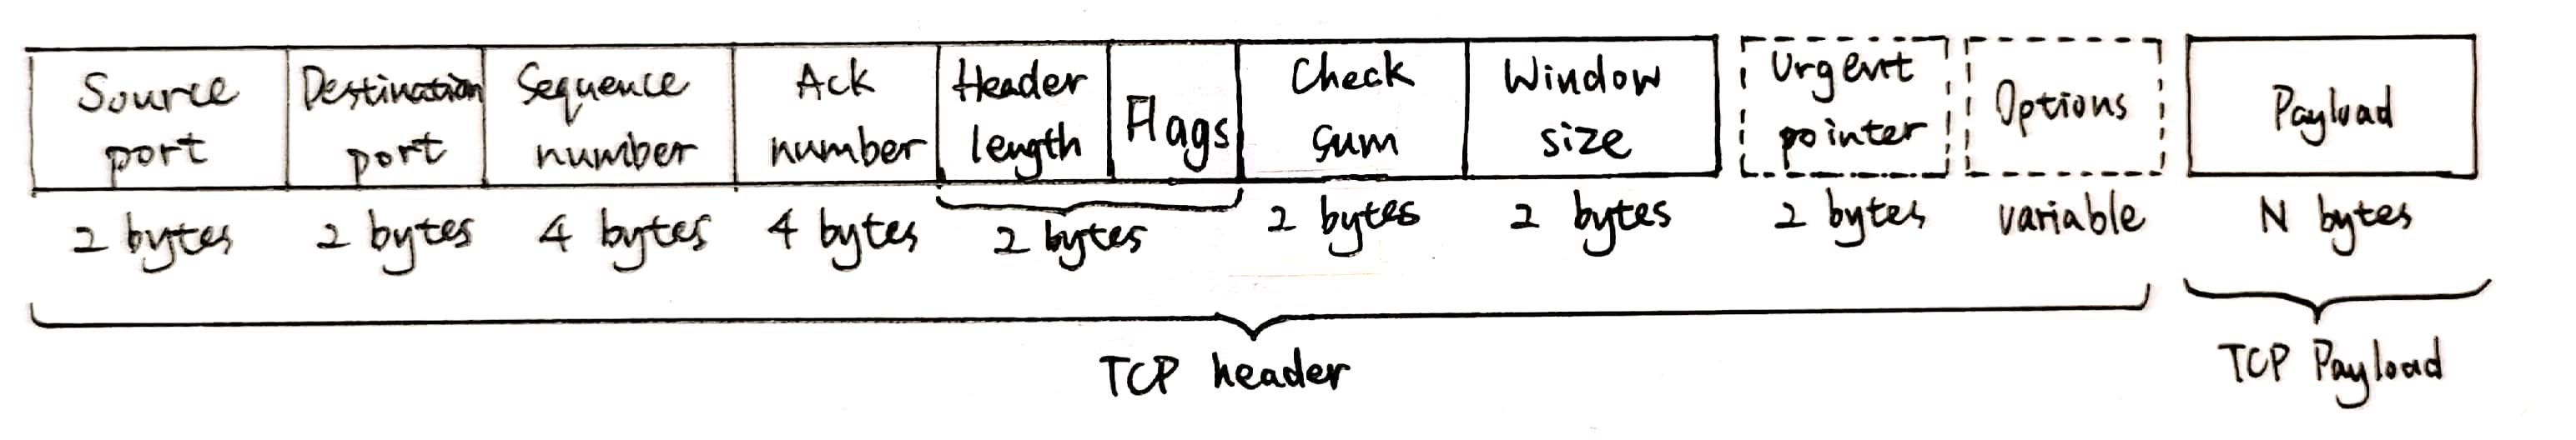
\includegraphics[scale=0.5]{1.jpg}
\caption{My screenshot of a packet trace of wget traffic.}
\end{figure}
A screenshot of a packet trace of “wget http://umji.sjtu.edu.cn” traffic is shown in Figure 1. These packets are all colored green in Wireshark, indicating that the fetch is successful. The packet selected in the figure is a packet whose Protocol column is “HTTP” and Info column is a GET request. It is the packet that carries the web (HTTP) request sent from my computer to the server.

\section{Step 2: Inspect the Trace}
\begin{figure}[htbp]
\centering
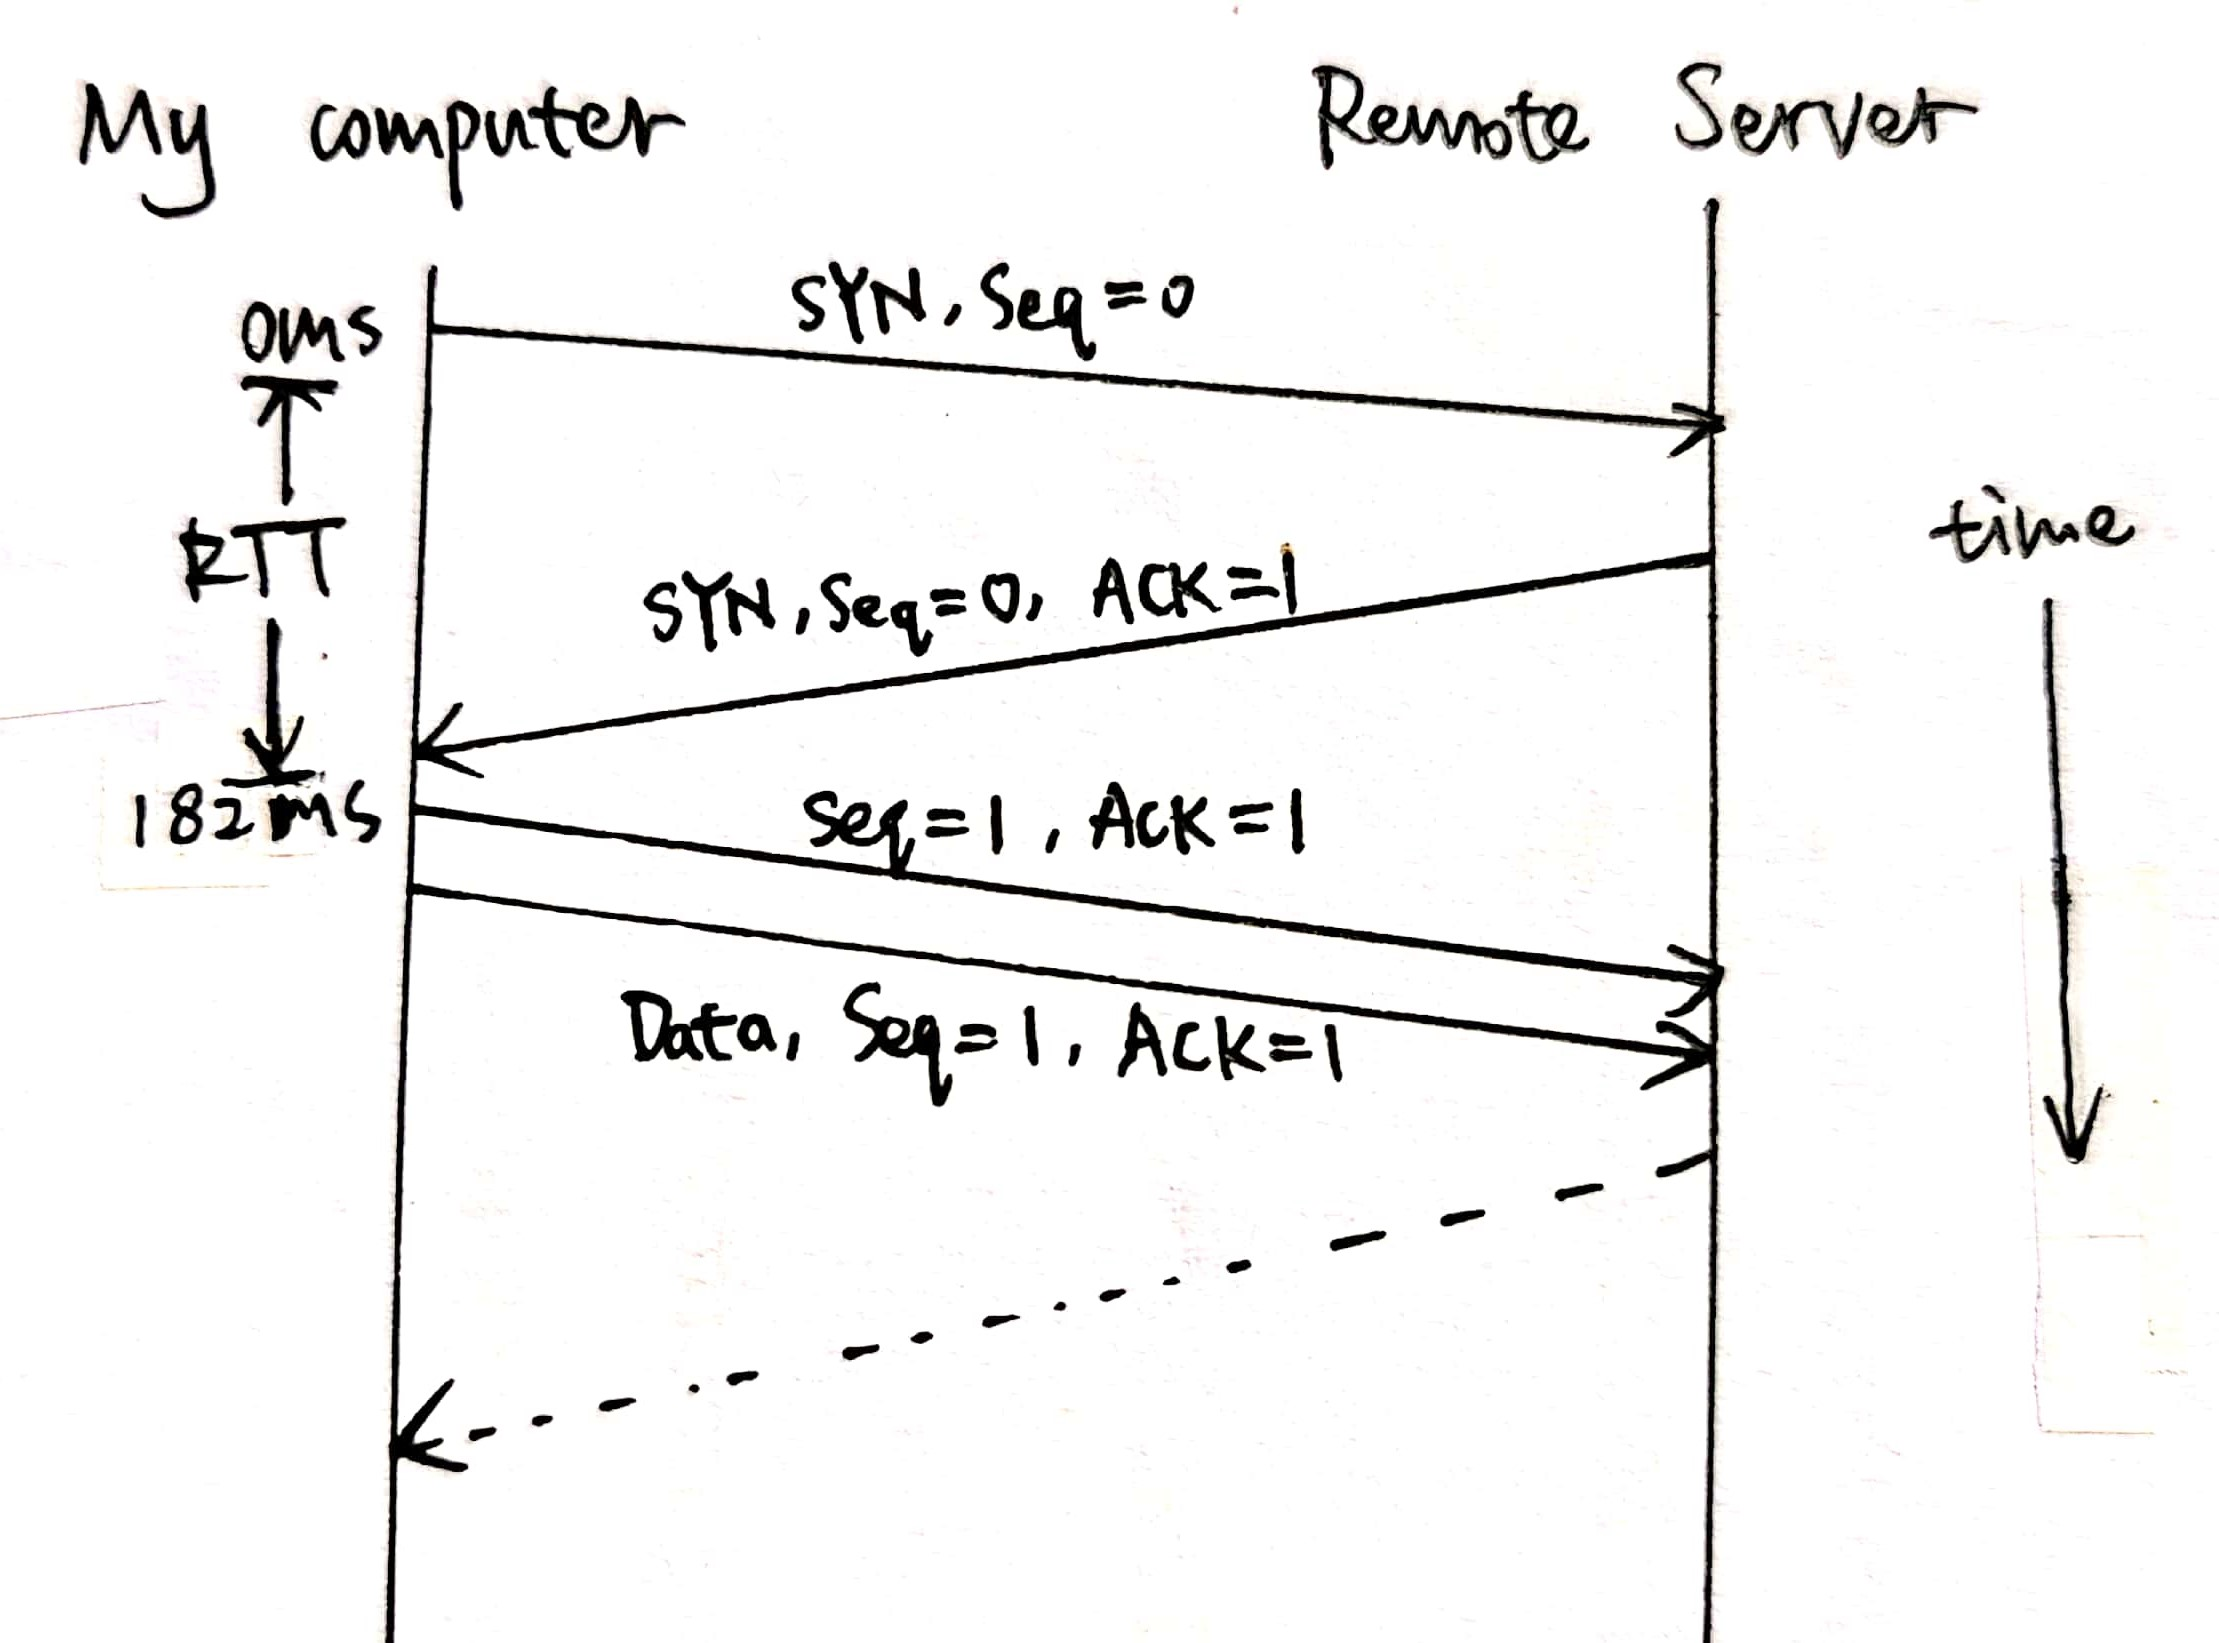
\includegraphics[scale=0.5]{2.jpg}
\caption{My screenshot of a HTTP “200 OK” response.}
\end{figure}
A screenshot of a HTTP “200 OK” response is shown in Figure 2. This packet is the response from the server to my computer. The “200 OK” in the Info field indicates that the web fetch is successful.

\section{Step 3: Packet Structure}
\begin{figure}[htbp]
\centering
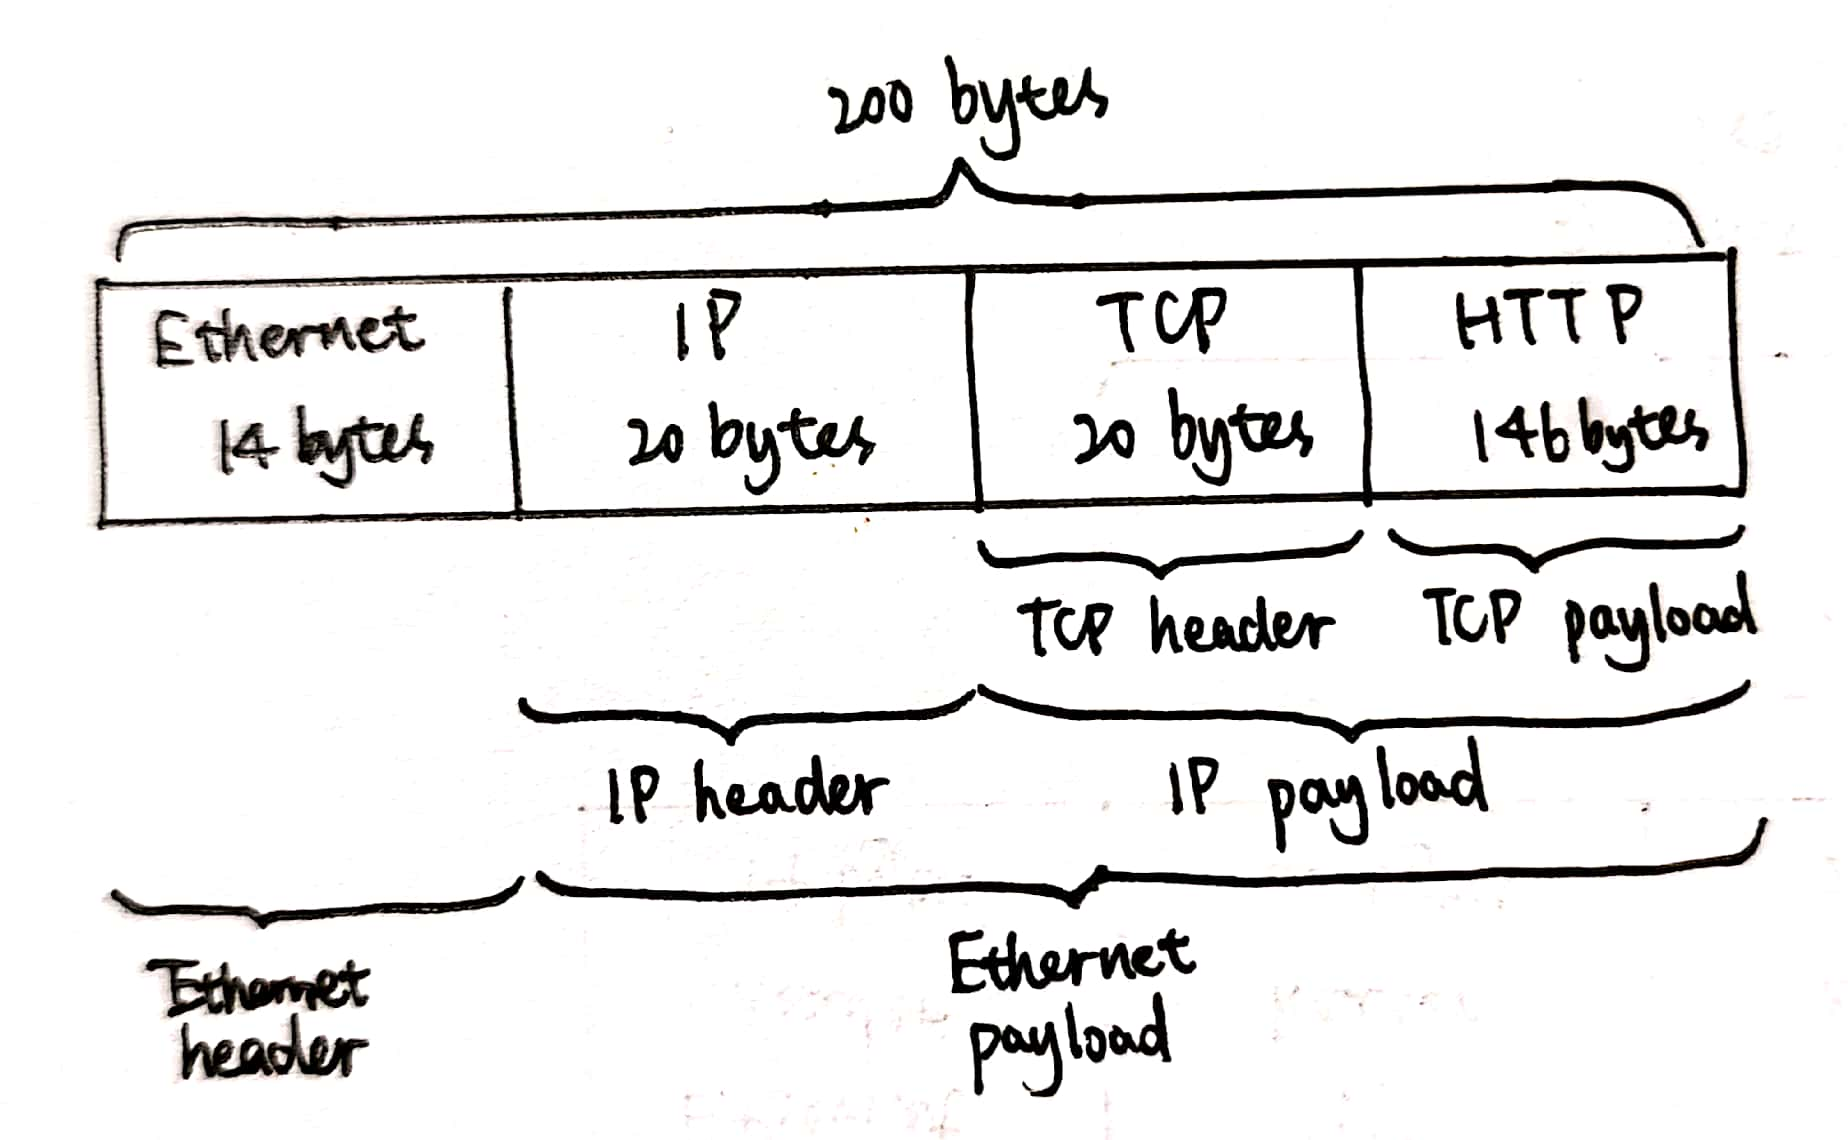
\includegraphics[scale=0.15]{3.jpg}
\caption{The packet structure of an HTTP GET packet.}
\end{figure}

\section{Step 4: Protocol Overhead}
\begin{figure}[htbp]
\centering
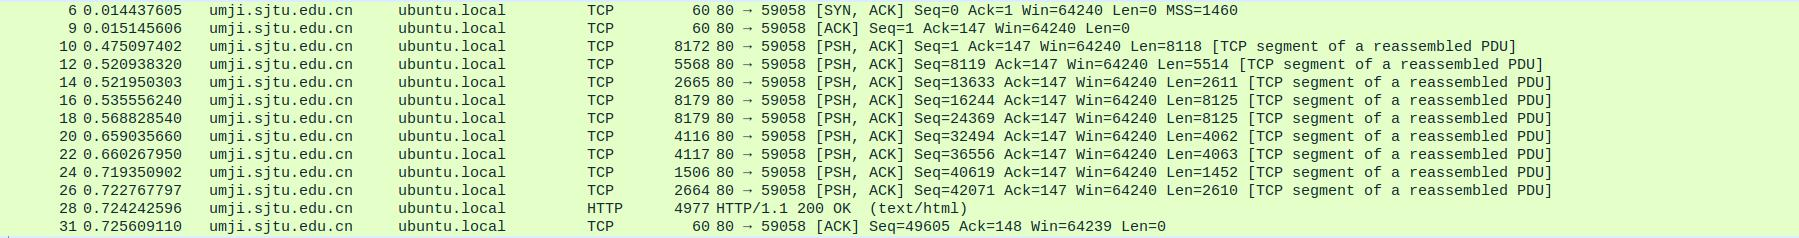
\includegraphics[scale=0.5]{4.jpg}
\caption{A screenshot of the packets in the download direction.}
\end{figure}
As shown in Figure 4, the download packets start with a short TCP packet described as a SYN ACK, which denotes the beginning of a connection. Then, there are 10 longer packets, of which the last one is an HTTP packet. Lastly, there is a short TCP packet indicating the end of the connection.
\par
To calculate download protocol overheads, we focus on the 10 longer packets in the middle. For each packet, the overheads exist in the form of Ethernet / IP / TCP headers, which is 14+20+20=54 bytes. So there are totally $54\times10=540$ bytes of download protocol overheads. The overhead rate can be calculated as:
\begin{align*}
Overhead\ Rate &=\dfrac{54\times10}{8172+5568+2665+8179+8179+4116+4117+1506+2664+4977}\\
&=\dfrac{540}{50143}\\
&=1.077\%
\end{align*}
which, in my opinion, is not very significant and is fairly acceptable.

\section{Step 5: Demultiplexing Keys}
\begin{enumerate}
\item
The demultiplexing key that tells Ethernet the next higher layer is IP is the Type field. The value 0x0800 is used in this field to indicate “IP”.
\item
The demultiplexing key that tells IP the next higher layer is TCP is the Protocol field. The value 0x06 is used in this field to indicate “TCP”.
\end{enumerate}

\section{Explore on my own}
\begin{enumerate}
\item
The packet is destined to the TCP protocol entity of the receiving computer instead of entities that have HTTP. It is only exchanged between TCP entities in a peer-to-peer style to maintain their connection. Therefore, it does not need to carry higher-layer data.
\item
The drawing of the first TCP packet will have an HTTP header inside while the drawing of the last TCP packet will only have HTTP payload data but no HTTP header. Moreover, if the HTTP header is very long, then the first drawing will only have HTTP header but no HTTP payload data.
\item
If a lower layer adds encryption, it will rewrite its payload and append its header. Correspondingly, the payload of higher protocols will be inaccessible when the packet is transmitted. It will only be accessible after the receiving end decrypts the message.
\item
If a lower layer adds compression, it will rewrite its payload and append its header. The new payload data will be shorter than the original one. Correspondingly, the payload of higher protocols will be inaccessible when the packet is transmitted. It will only be accessible after the receiving end decompresses the message.
\end{enumerate}


\end{document}